\DiaryEntry{Linear Algebra - QR Decomposition, Givens Rotations}{2020-01-06}{Linear Algebra}

The Householder transform zeros out all matrix elements but one in a row. On contrast, the Givens rotation zeros out one matrix element. 

\subsection{Two-dimensional Case}

Let's start with a simple two-dimensional case. We have a vector

\bee
\xbf = \begin{pmatrix} x_1 \\ x_2 \end{pmatrix}
\eee

and a rotation matrix

\bee
\Rbf = \begin{pmatrix} \cos \phi & \sin\phi \\ -\sin\phi & \cos\phi \end{pmatrix}
\eee

Left-multiplying $\xbf$ with $\Rbf$ yields

\bee
\Rbf \xbf = \begin{pmatrix} x_1 \cos\phi - x_2 \sin\phi \\ -x_1 \sin\phi + x_2 \cos\phi \end{pmatrix}
\eee

We can choose the rotation angle $\phi$ in such a way that the y-component becomes zero.

\bee
-x_1 \sin\phi + x_2 \cos\phi = 0 \rightarrow \frac{\sin\phi}{\cos\phi} = - \frac{x_2}{x_1}
\eee

which can be solved for $\phi$,

\bee
\phi = - \arctan \frac{x_2}{x_1}
\eee

As an example, consider the following Julia session where we zero the second element of $\xbf$:

\begin{verbatim}
x=[2;5]
2-element Array{Int64,1}:
 2
 5
phi=atan(-5/2)
-1.1902899496825317
R=[cos(phi) -sin(phi); sin(phi) cos(phi)]
2×2 Array{Float64,2}:
  0.371391  0.928477
 -0.928477  0.371391
R*x
2-element Array{Float64,1}:
 5.385164807134504    
 2.220446049250313e-16
\end{verbatim}


\subsection{General Case}

We next extend the rotation into higher dimensions. We consider rotations which change 2 coordinates and leave the other unchanged; i.e. rotations along the axes. In case of three dimensions, there are three such rotations: (i) Rotation in the $x-y$ plane, leaving the $z$-component unchanged, (ii) rotation in the $x-z$ plan, leaving the $y$-component unchanged, and (iii) rotation in the $y-z$ plane, leaving the $x$-component unchanged.

A matrix which rotates in the $i-k$ plane has the following form

\begin{figure}[hbt!]
\centering
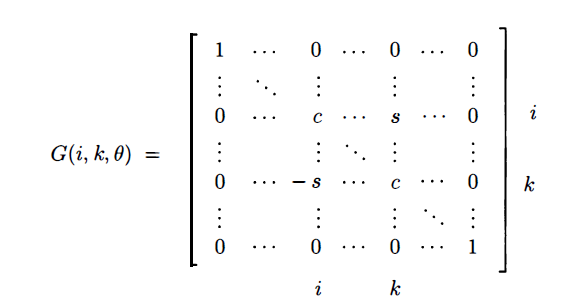
\includegraphics[scale=0.7]{images/qr_givens.png}
\end{figure}

where $c = \cos \theta$ and $s = \sin \theta$ and $\theta$. Left-multiplying a matrix $\Abf$ by $\Gbf(i,k,\theta)$ modifies rows $i$ and $k$ of the matrix $\Abf$ and \emph{leaves all other rows unchanged}.

Since we want to zero out several element of $\Abf$, we need to apply several Givens rotation matrices; one rotation for each element to zero. In order to prevent that later rotations affect previous ones, the rows $i$ and $j$ f each rotation and the order of rotations must be chosen carefully.

We show the process at the example of a $3 \times 3$ matrix

\bee
\Abf = \begin{pmatrix}
  a_{1,1} & X & X \\
  a_{2,1} & a_{2,2} & X \\
  a_{3,1} & a_{3,2} & X
\end{pmatrix}
\eee

We first zero $a_{3,1}$ by a Givens rotation $\Gbf(2,3,\theta_1)$; i.e. we perform a rotation in the $y-z$ plan by an angle chosen as

\bee
\theta_1 = \frac{a_{3,1}}{a_{2,1}}
\eee

We continue in the first column and go upwards to zero $a_{2,1}$ by a rotation in the $x-y$ plan, $\Gbf(1,2,\theta_2)$ with

\bee
\theta_2 = \frac{a_{2,1}}{a_{1,1}}
\eee

After applying this second rotation, we are left with

\bee
\Gbf(1,2,\theta_2) \Gbf(2,3,\theta_1)\Abf = \begin{pmatrix}
  a'_{1,1} & X & X \\
  0 & a'_{2,2} & X \\
  0 & a'_{3,2} & X
\end{pmatrix}
\eee

Note that due to the rotatons, matrix elements will have changed (in particular the elements $a_{1,1}, a_{2,2}, a_{3,2}$). As last element, we need to zero $a_{3,2}$. We do this by a Givens rotation $\Gbf(2,3,\theta_3)$; note that this matrix has the same form as the one used for zeroing $a_{3,1}$ but uses a different angle

\bee
\theta_3 = \frac{a'_{3,2}}{a'_{2,2}}
\eee

Note that this rotation affects all elements in rows $2$ and $3$; however $a_{3,1}$ and $a_{2,1}$ are already zero and are therefore not changed by this rotation.

Had we used $\Gbf(1,3,\theta_3)$ for this last rotation, we could chose $\theta_3$ such that $a_{3,2}$ becomes zero; however $a_{1,1}$ is non-zero and this would cause $a_{3,1}$ to become non-zero again due to the rotation. 

In case of a general $m \times m$ matrix, the sequence of Givens rotations has the following form

\bee
\Gbf(m-1,m,\theta_1) \Gbf(m-2,m-1, \theta_2) \cdots \Gbf(1,2,\theta_{m-1}) \Gbf(m-1,m,\theta_m) \cdots \Gbf(2,2,\theta)
\eee

We then have

\bee
\Gbf(m-1,m,\theta_1) \Gbf(m-2,m-1, \theta_2) \cdots \Gbf(1,2,\theta_{m-1}) \Gbf(m-1,m,\theta_m) \cdots \Gbf(2,2,\theta) \Abf = \Rbf
\eee

and since the $\Gbf$ matrices are orthonormal, we can easily invert them and arrive at

\bee
\Abf = \Gbf(2,2,\theta)^T \cdots \Gbf(m-2,m-1, \theta_2)^T \Gbf(m-1,m,\theta_1)^T\Rbf
\eee





\subsection{Three-dimensional Example}

We will demonstrate the process described above with the example of a $3 \times 3$ matrix $\Abf$

\bee
\Abf = \begin{pmatrix} 1 & 4 & 6 \\ -2 & 5 & 10 \\ 4 & 2 & -5 \end{pmatrix}
\eee

This is done in the following Julia session (code is \href{https://github.com/ClemensFMN/JuliaStuff/blob/master/qr_givens.jl}{here}).

\begin{verbatim}
using LinearAlgebra

julia> A=[1 4 6;-2 5 10;4 2 -5]
3×3 Array{Int64,2}:
  1  4   6
 -2  5  10
  4  2  -5

function getR(theta,m,i,j)
    R = Matrix(1.0I,m,m)
    R[i,i] = 0
    R[j,j] = 0
    R[j,j]= cos(theta)
    R[j,i] = sin(theta)
    R[i,j] = -sin(theta)
    R[i,i] = cos(theta)
    return R
end
\end{verbatim}

We first start zeroing out $a_{3,1}$

\begin{verbatim}
i=2
j=3
k=1
theta = atan(- A[j,k]/A[i,k])
R1 = getR(theta,3,i,j)
julia> R1 = getR(theta,3,i,j)
3×3 Array{Float64,2}:
 1.0  0.0        0.0     
 0.0  0.447214  -0.894427
 0.0  0.894427   0.447214
julia> A=R1*A
3×3 Array{Float64,2}:
  1.0          4.0       6.0    
 -4.47214      0.447214  8.94427
  4.44089e-16  5.36656   6.7082
\end{verbatim}

Next is zeroing $a_{2,1}$

\begin{verbatim}
i=1
j=2
k=1
theta = atan(- A[j,k]/A[i,k])
julia> R2 = getR(theta,3,i,j)
3×3 Array{Float64,2}:
 0.218218  -0.9759    0.0
 0.9759     0.218218  0.0
 0.0        0.0       1.0
julia> A=R2*A
3×3 Array{Float64,2}:
  4.58258      0.436436  -7.41941
 -1.11022e-16  4.00119    7.8072 
  4.44089e-16  5.36656    6.7082 
\end{verbatim}

And finally, we zero $a_{3,2}$

\begin{verbatim}
i=2
j=3
k=2
theta = atan(- A[j,k]/A[i,k])
julia> R3 = getR(theta,3,i,j)
3×3 Array{Float64,2}:
 1.0   0.0       0.0     
 0.0   0.597729  0.801699
 0.0  -0.801699  0.597729
julia> A = R3*A
3×3 Array{Float64,2}:
 4.58258      0.436436  -7.41941
 2.89664e-16  6.69399   10.0445 
 3.54451e-16  0.0       -2.24934
\end{verbatim}

We are done and have the following connections to the QR decomposition: $\Abf = \Rbf_1^T \Rbf_2^T \Rbf_3^T \Rbf^T = \Qbf \Rbf$ with $\Qbf = \Rbf_1^T \Rbf_2^T \Rbf_3^T$ which we can compare with Julia's QR function

\begin{verbatim}
julia> R1'*R2'*R3'
3×3 Array{Float64,2}:
  0.218218  0.583323  -0.782378
 -0.436436  0.775393   0.456387
  0.872872  0.241866   0.423788
julia> A
3×3 Array{Float64,2}:
 4.58258      0.436436  -7.41941
 2.89664e-16  6.69399   10.0445 
 3.54451e-16  0.0       -2.24934

julia> qr(A)
LinearAlgebra.QRCompactWY{Float64,Array{Float64,2}}
Q factor:
3×3 LinearAlgebra.QRCompactWYQ{Float64,Array{Float64,2}}:
 -0.218218  -0.583323  -0.782378
  0.436436  -0.775393   0.456387
 -0.872872  -0.241866   0.423788
R factor:
3×3 Array{Float64,2}:
 -4.58258  -0.436436    7.41941
  0.0      -6.69399   -10.0445 
  0.0       0.0        -2.24934
\end{verbatim}

The results are the same apart from some signs.


%%% Local Variables:
%%% mode: latex
%%% TeX-master: "journal"
%%% End:
